\documentclass[a4paper,12pt]{article}
\usepackage[utf8]{inputenc}
\usepackage[french]{babel}
\usepackage[T1]{fontenc}
\usepackage[top=2cm,bottom=2cm,left=2cm,right=2cm]{geometry}
\usepackage{graphicx}
\usepackage{wrapfig}
\usepackage{url}
\usepackage{color}

\begin{document}

\begin{titlepage}
	\begin{center}
		\Large{Année universitaire 2016-2017}\\
		\Large{Université de Caen Normandie}\\[1cm]
		
		\huge{Rapport sur les snippets}\\
		\vspace{3cm}
		
		Théo Sarrazin
		
	\normalsize{\textit{ ~ L2 Informatique}}\\
		\medskip
		\vspace{2cm}
				
	\end{center}
\end{titlepage}

\tableofcontents
\newpage

\section{Snippets}
	
	\subsubsection{Les snippets : explication}

		Les snippets sont des bouts de code qui sont réutilisables d'un projet à un autre (comme les conditions, les boucles et les définitions de fonction par example). Dans notre IDE nous utilisons des mots clés que l'on associes à ces bouts de code. Lorsque l'on tape un des mots clés puis que l'on presse la touche \textbf{tabulation}, le mot clé est remplacé par le bout de code qui correspond.

	\subsubsection{Intergration des bouts de code dans l'IDE}

		\subsubsubsection{Utilisation du JSON}

			Pour l'intégration des snippets dans l'IDE, nous avons utilisés des fichier JSON, qui contiennent des dictionnaires avec comme clé le mot clé qui correspond au bout de code et en valeur le dit bout de code, suivit de nombre de ligne de le cursor doit remonter, puis le nombre de charactère char que le cursor doit parcourir vers la droite pour être à l'emplacement voulu. De plus nous avons un fichier JSON par language (C, python, etc ... )

			\begin{figure}[h!]
				\begin{center}
					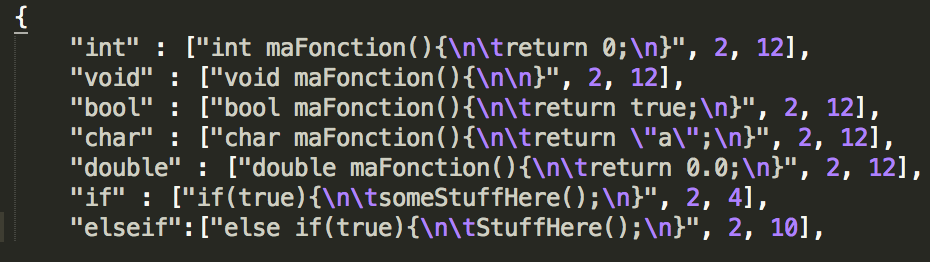
\includegraphics[scale=1]{imgs/exempleJSON}
					\caption{Extrait du fichier JSON pour le language C}
				\end{center}
			\end{figure}

		\subsubsubsection{Connection entre le JSON et l'IDE}

			Pour capturer l'appuie sur la touche \textbf{tabulation}, nous utilisons le méthode \textbf{keyPressEvent} de notre classes \textbf{Editeur}. Cette méthode est appelée à l'appuie sur une des touches du clavier. Par la suite, si la touche est la touche \textbf{tabulation}, nous parsons le JSON pour avoir touts les couples mot clé - bout de code. Puis en fonction du mot placé au niveau du curseur, on le remplace ou non par le bout de code correspondant.

			\begin{figure}[h!]
				\begin{center}
					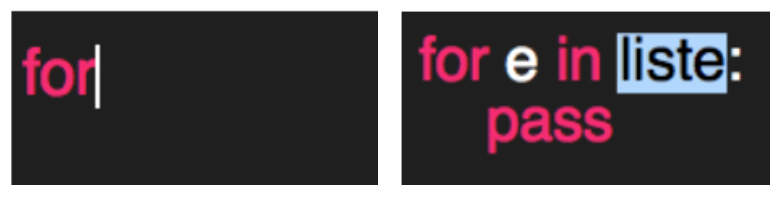
\includegraphics[scale=0.7]{imgs/exampleFor}
					\caption{Exemple d'utilisation des snippets avec une boucle for en Python}
				\end{center}
			\end{figure}

\section{Compilateur}

	\subsection{Compilateurs utilisés}

		Pour notre IDE, nous avons utilisés le compilateur \textbf{GCC}, pour compiler les projets de type \textbf{C}. Mais nous utilisons aussi les interpréteur de python afin d'interpréter les projets de type \textbf{Python}. Par la suite, pour chaque nouveaux languages il nous suffit d'utiliser le bon compilateur ou le bon interpréteur.
		
	\subsection{Integration de \textbf{GCC} à notre IDE}

		Pour utilisé \textbf{GCC} avec notre IDE nous avons créé une fenêtre de configuration afin de permettre à l'utilisateur de choisir la configuration adéquate à la compilation de son projet.

			\begin{figure}[h!]
				\begin{center}
					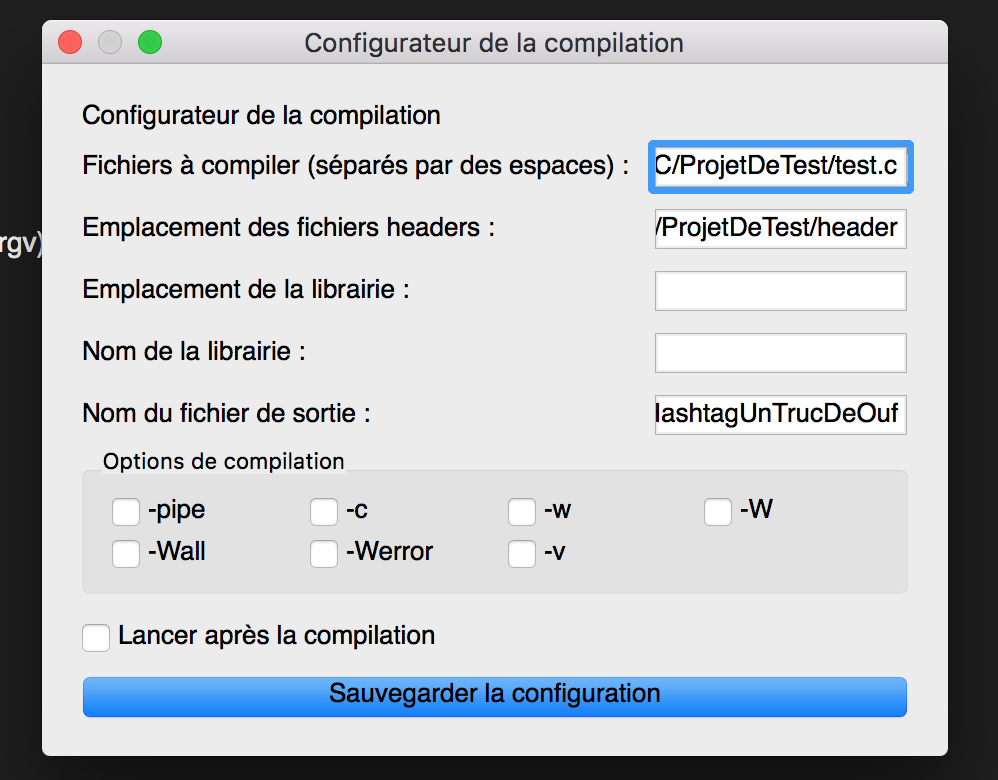
\includegraphics[scale=0.7]{imgs/fenCompEx}
					\caption{Fenêtre de configuration de GCC}
				\end{center}
			\end{figure}

		Par la suite, chaque information de cette fenêtre est convertie en une chaîne de caractère du type : 

		gcc /Users/theosarrazin/workplaceC/ProjetDeTest/test.c  -I /Users/theosarrazin/workplaceC/

		ProjetDeTest/header -o MonExecutable

		Cette chaîne de caractère est stockée dans le fichier XML de configuration du projet.

		Par la suite on exécute cette ligne de commande, puis on récupère sur la sortie d'erreurs les eventuelles erreurs afin de pouvoir les afficher à l'utilisateur après les avoir parsé pour avoir un bon formatage.

		\newpage

			\begin{figure}[h!]
				\begin{center}
					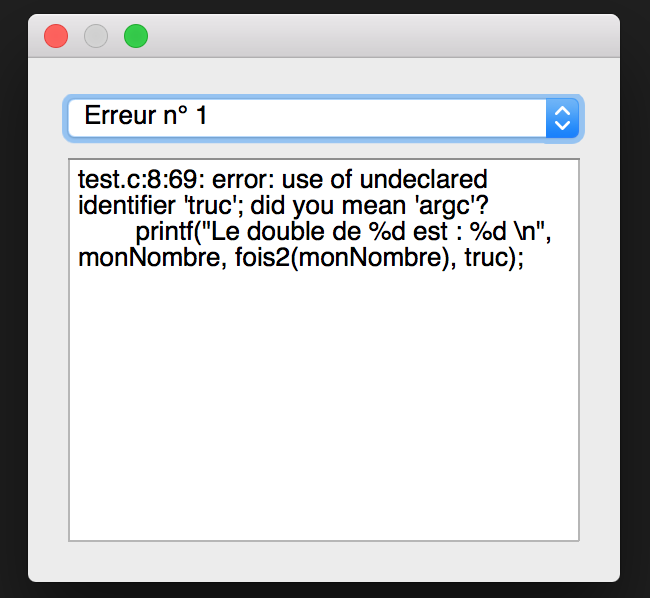
\includegraphics[scale=0.7]{imgs/fenErreurEx}
					\caption{Affichage des erreurs de GCC dans l'IDE}
				\end{center}
			\end{figure}

		Pour la partie interpréteur la demarche est identique. 

\section{Cache}

	\subsection{Utilité du cache}

		Afin de pouvoir faire de la coloration, nous avons utilisés \textbf{Lex} mais pour les fichiers de plusieurs 100\up{ène} de lignes \textbf{Lex} prend plusieurs secondes pour nous donner la listes des tokens du fichier. Nous avons donc décidé d'utiliser un fichier de cache afin de ne pas utiliser \textbf{Lex} pour colorer des lignes que nous avons déjà coloré de manière ultérieure.

	\subsection{Intégration du cache dans l'IDE}

		Pour le cache, nous avons décidé d'utiliser un fichier JSON pour l'enregistrer. Le fonctionnement est assez simple la clé est le bout de code que l'on donne à \textbf{Lex} et la valeur est la réponse de ce dernier. Par la suite il nous reste plus qu'à utiliser les valeurs du fichier JSON à la place de \textbf{Lex}

			\begin{figure}[h!]
				\begin{center}
					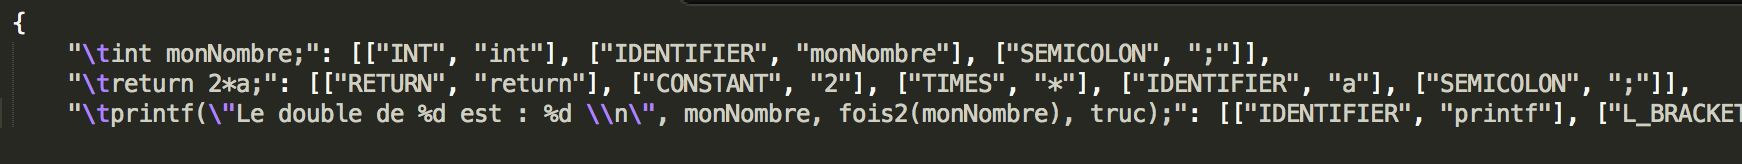
\includegraphics[scale=0.5]{imgs/exempleJsonCache}
					\caption{Extrait d'un JSON contenant le cache}
				\end{center}
			\end{figure}

		Grâce au cache nous avons un gain de temps considérable sur l'ouverture des documents.
	
\end{document}